 % -*- root: ../../twm.tex -*-

 \section{Processing Data}
\begin{frame}
    \frametitle{Processing}
    \begin{itemize}
        \item Often depends on theoretical model
        \begin{itemize}
            \item Time series models for stock returns
            \item Example 2
        \end{itemize}
        \item Just a side note in scientific articles
        \begin{itemize}
            \item Well established ``gold standard'' processing for many domains
            \item No scientific news value
        \end{itemize}
    \end{itemize}
\end{frame}

\begin{frame}
    \frametitle{Part of Speech Tagging}
\begin{itemize}
    \item More than nouns, verbs, adjectives
        \begin{itemize}
        \item Penn Treebank: 45 tags
        \item Brown Corpus: 87 tags
        \end{itemize}
        \end{itemize}
\begin{itemize}
    \item Useful for
        \begin{itemize}
        \item Information retrieval
        \item Word-sense disambiguation
        \item Shallow parsing of names and other named entities
        \end{itemize}
     \end{itemize}
     \begin{itemize}
    \item Math Tagging, \textcolor{iseblue}{Kristianto et al (2012)}
         \begin{itemize}
    \item Extract mathematical definitions
    \item Pattern matching and machine learning
\end{itemize}
\end{itemize}

\end{frame}


\begin{frame}
    \frametitle{Example: Beer Review}
\begin{spacing}{1.6}
    An OK lager. Light, crisp, but nothing special. Stacked against the great pilsners of the world or similar offerings, this beer is mediocre. But still solid enough to put it head and shoulders above any macro. 
\end{spacing}

\end{frame}


\begin{frame}
    \frametitle{Nouns}
\begin{spacing}{1.6}
    An OK \textbf{\textcolor{isered}{lager}}. \textbf{\textcolor{isered}{Light}}, crisp, but \textbf{\textcolor{isered}{nothing}} special. Stacked against the great \textbf{\textcolor{isered}{pilsners}} of the \textbf{\textcolor{isered}{world}} or similar \textbf{\textcolor{isered}{offerings}}, this \textbf{\textcolor{isered}{beer}} is mediocre. But still solid enough to put it \textbf{\textcolor{isered}{head}} and \textbf{\textcolor{isered}{shoulders}} above any \textbf{\textcolor{isered}{macro}}.
\end{spacing}

\vspace{-10pt}
\begin{flushright}
    \textbf{\textcolor{isered}{NOUN}}
\end{flushright}

\vspace{-10pt}
\begin{itemize}
\item Which topic?
\item Which beer category? Lager, pilsner
\end{itemize}
\end{frame}


\begin{frame}
    \frametitle{POS Tagging is not perfect}
\begin{spacing}{1.6}
    An OK \textbf{\textcolor{isered}{lager}}. \textbf{\mybox{\textcolor{isered}{Light}}}, crisp, but \textbf{\textcolor{isered}{nothing}} special. Stacked against the great \textbf{\textcolor{isered}{pilsners}} of the \textbf{\textcolor{isered}{world}} or similar \textbf{\textcolor{isered}{offerings}}, this \textbf{\textcolor{isered}{beer}} is mediocre. But still solid enough to put it \textbf{\textcolor{isered}{head}} and \textbf{\textcolor{isered}{shoulders}} above any \textbf{\textcolor{isered}{macro}}.
\end{spacing}

\vspace{-10pt}
\begin{flushright}
    \textbf{\textcolor{isered}{NOUN}}
\end{flushright}

\vspace{-10pt}
\begin{itemize}
\item Which topic? Beer
\item Which beer category? Lager, pilsner
\end{itemize}

\end{frame}


\begin{frame}
    \frametitle{\textcolor{iseblue}{Verbs}}
    \label{review_verbs}
\begin{spacing}{1.6}
    An OK \textbf{\textcolor{isered}{lager}}. \textbf{\textcolor{isered}{Light}}, crisp, but \textbf{\textcolor{isered}{nothing}} special. \textbf{\textcolor{iseblue}{Stacked}} against the great \textbf{\textcolor{isered}{pilsners}} of the \textbf{\textcolor{isered}{world}} or similar \textbf{\textcolor{isered}{offerings}}, this \textbf{\textcolor{isered}{beer}} \textbf{\textcolor{iseblue}{is}} mediocre. But still solid enough to \textbf{\textcolor{iseblue}{put}} it \textbf{\textcolor{isered}{head}} and \textbf{\textcolor{isered}{shoulders}} above any \textbf{\textcolor{isered}{macro}}.
\end{spacing}

\vspace{-10pt}
\begin{flushright}
    \textbf{\textcolor{isered}{NOUN}}, \textbf{\textcolor{iseblue}{VERB}}
\end{flushright}

\begin{itemize}
\item Relationships between nouns $\; \;$\hyperlink{dependency_tree}{\beamerbutton{Dependency Tree}}
\item Here: not very informative
\end{itemize}

\end{frame}

\begin{frame}
    \frametitle{\textcolor{isegreen}{Adjectives}}
\begin{spacing}{1.6}
    An \textbf{\textcolor{isegreen}{OK}} \textbf{\textcolor{isered}{lager}}. \textbf{\textcolor{isered}{Light}}, \textbf{\textcolor{isegreen}{crisp}}, but \textbf{\textcolor{isered}{nothing}} \textbf{\textcolor{isegreen}{special}}. \textbf{\textcolor{iseblue}{Stacked}} against the \textbf{\textcolor{isegreen}{great}} \textbf{\textcolor{isered}{pilsners}} of the \textbf{\textcolor{isered}{world}} or \textbf{\textcolor{isegreen}{similar}} \textbf{\textcolor{isered}{offerings}}, this \textbf{\textcolor{isered}{beer}} \textbf{\textcolor{iseblue}{is}} \textbf{\textcolor{isegreen}{mediocre}}. But still \textbf{\textcolor{isegreen}{solid}} enough to \textbf{\textcolor{iseblue}{put}} it \textbf{\textcolor{isered}{head}} and \textbf{\textcolor{isered}{shoulders}} above any \textbf{\textcolor{isered}{macro}}.
\end{spacing}

\vspace{-10pt}
\begin{flushright}
    \textbf{\textcolor{isered}{NOUN}}, \textbf{\textcolor{iseblue}{VERB}}, \textbf{\textcolor{isegreen}{ADJ}}
\end{flushright}

\begin{itemize}
\item What is the opinion? OK, solid, (nothing) special, mediocre
\item How is something? Crisp
\end{itemize}
\end{frame}



\begin{frame}
    \frametitle{All Words}
\begin{figure}[htb]
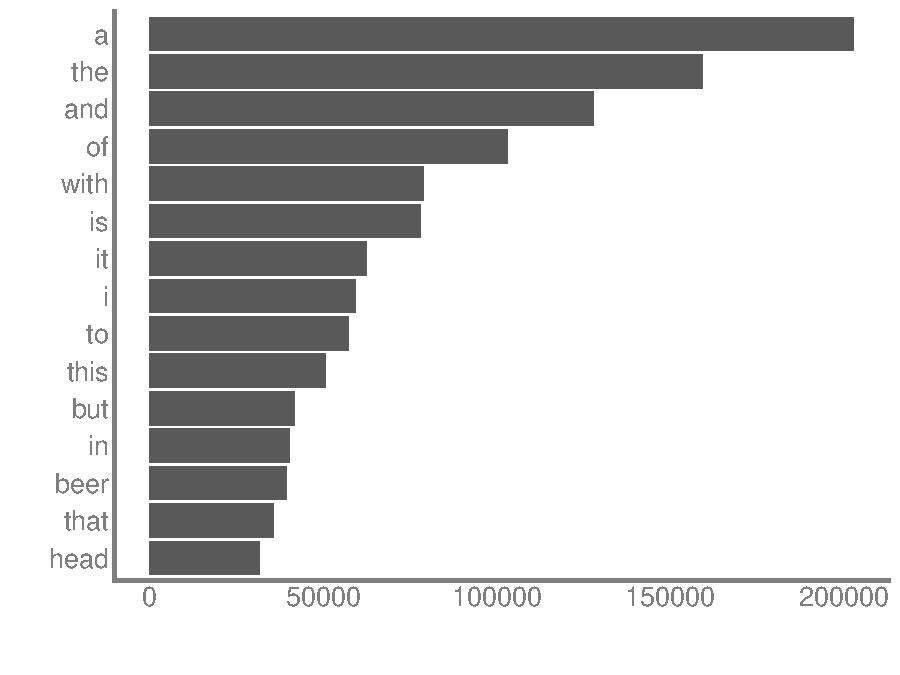
\includegraphics[scale=0.55,left]{img/figures/bar_words}
\end{figure}
\end{frame}

\begin{frame}
    \frametitle{Nouns}
\begin{figure}[htb]
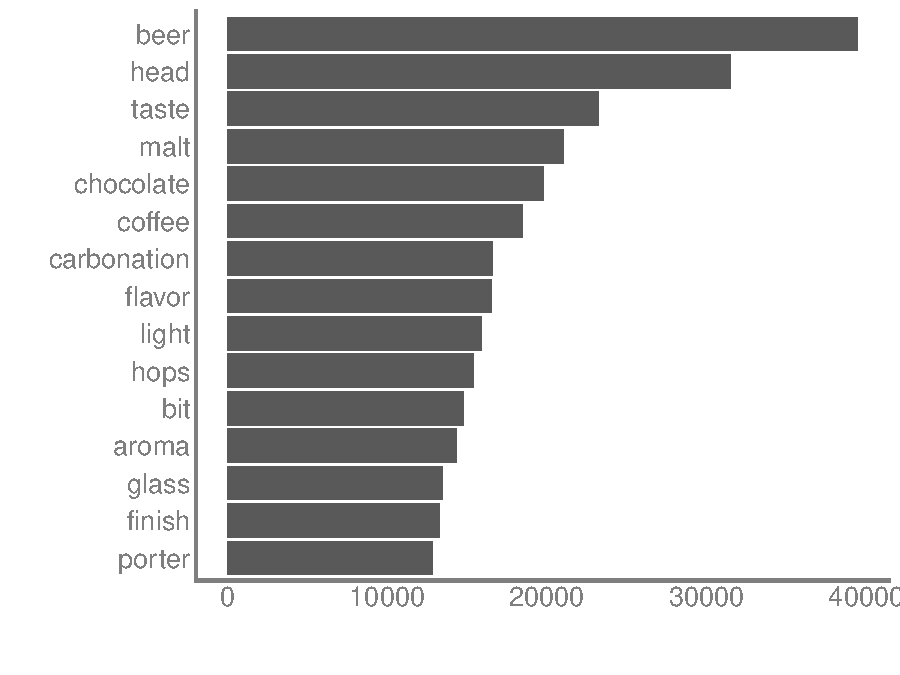
\includegraphics[scale=0.55,left]{img/figures/bar_nouns}
\end{figure}
\end{frame}

\begin{frame}
    \frametitle{Adjectives}
\begin{figure}[htb]
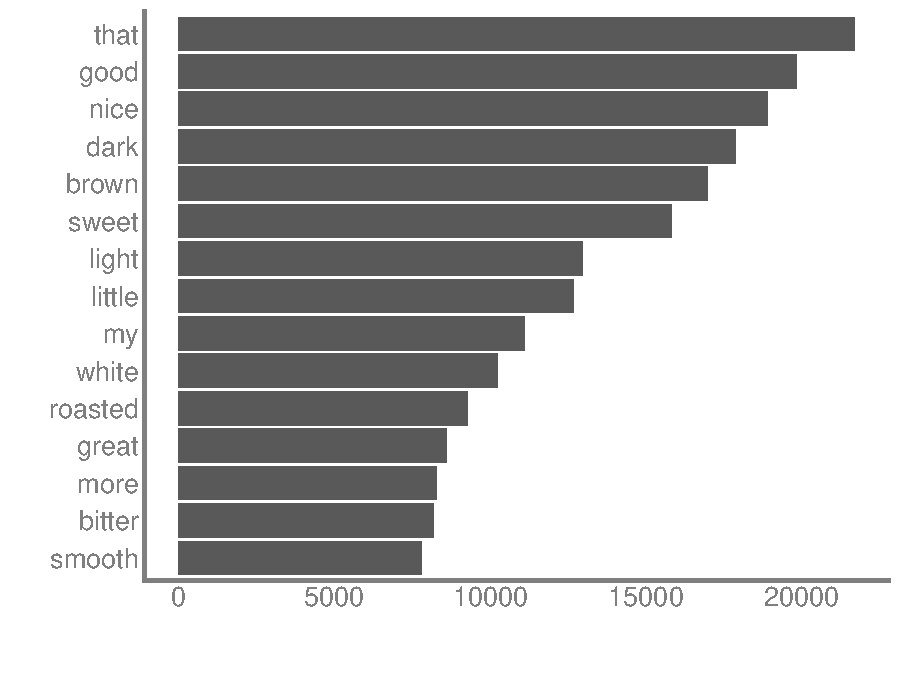
\includegraphics[scale=0.55,left]{img/figures/bar_adj}
\end{figure}
\end{frame}


\begin{frame}
    \frametitle{Text Normalization: Basics}
\begin{spacing}{1.6}
    [ (an, ok lager), (light, crisp, but, nothing, special), (stacked, against, the, great, pilsners, of, the, world, or, similar, offerings, this, beer, is, mediocre), (but, still, solid, enough, to, put, it, head, and, shoulders, above, any, macro) ]
\end{spacing}
\vspace{10pt}
\begin{itemize}
\item Lowercase
\item Removal of non alphabetic characters
\item Word and sentence lemmatization
\end{itemize}
\end{frame}

\begin{frame}
    \frametitle{Text Normalization: Lemmatization}
\begin{spacing}{1.6}
    (stacked, stack), (pilsners, pilsner) \\
    (offerings, offering), (is, be) \\
    (it, -PRON-), (shoulders, shoulder)
\end{spacing}
\vspace{10pt}
\begin{itemize}
\item Map a word to its canonical form
\item Alternative to stemming
\end{itemize}
\end{frame}

\begin{frame}
    \frametitle{Text Normalization: Special Cases}
\begin{itemize}
\item Dates
\begin{itemize}
\item Canonical form: 22.11.2017 $\rightarrow$ 11/22/2017
\item Relative to absolute: Yesterday $\rightarrow$ 11/22/2017
\end{itemize}
\item Abbreviations
\begin{itemize}
\item Common: United States of America $\rightarrow$ USA
\item Specific: ordinary least squares (OLS)
\end{itemize}
\item Numbers and units
\begin{itemize}
\item Hundred $\rightarrow$ 100
\item \$100 $\rightarrow$ 100\_dollar $\rightarrow$ 10000\_cent
\end{itemize}
\end{itemize}

\vspace{10pt}
What is the most important aspect of the domain?
\end{frame}

\begin{frame}
    \frametitle{Text Filtering: Noun Chunks}
\begin{spacing}{1.6}
    (An, OK, lager), (Light), (the, great pilsners) \\
    (the, world), (similar, offering), (this, beer) \\
    (it), (any, macro)
\end{spacing}
\vspace{10pt}
\begin{itemize}
\item Parse dependencies of nouns
\item Additional filtering for noun, adjective, verb combinations
\end{itemize}
\end{frame}

